\chapter{The Financial Smart Contract Web Client} \label{web-client}

One desired benefit of this project's contributions is the simplification of the creation of financial contracts. While the implementation of the financial smart contract program does simplify this, it is difficult to interact with due to the heavy serialization required in the smart contract's ABI. Rather than requiring users to learn and implement serialization/deserialization of all function parameters and return values, a web client has been implemented to facilitate this interaction and provide some additional functionality. \\

The web client facilitates the composition, deployment, and interaction/monitoring of financial smart contracts, as well as some basic evaluation functionality - a feature provided to reduce the risk of writing financial contracts and smart contracts. This chapter will describe the design and implementation of this web client. The implemented modules discussed in this chapter are depicted as a dependency graph in figure \ref{fig:client-block}. \\

\begin{figure}[h]
    \centering
    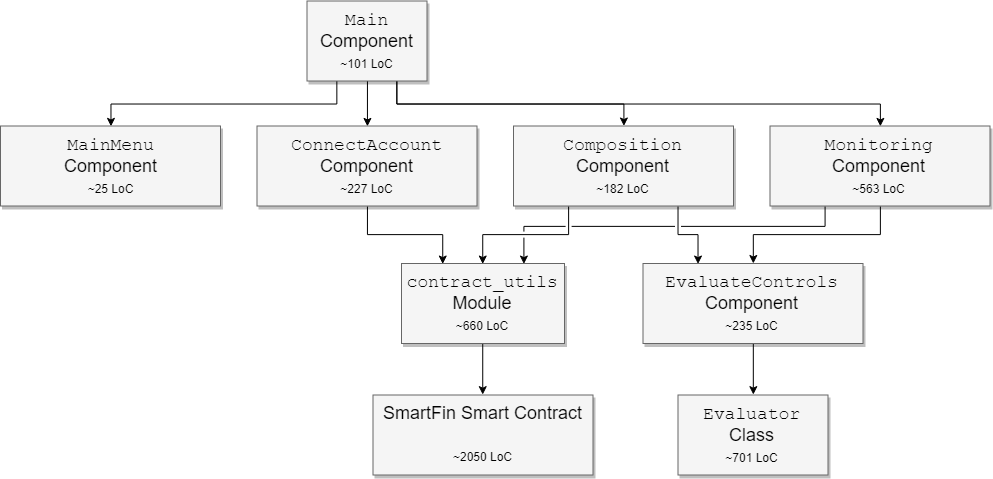
\includegraphics[width=\textwidth]{client-block.png}
    \caption{A dependency graph of the modules implemented for the web client, with their approximate \textit{Lines of Code} (not including tests). Small UI and data classes are not depicted. The SmartFin smart contract is described in chapters \ref{smart-contract-impl} and \ref{combinators-main}.}
    \label{fig:client-block}
\end{figure}


\section{The Design of the Web Client}

\subsection{Architecture}

From the beginning, the web client was designed around the use of \textit{React}\cite{react} - a JavaScript UI framework. Using some framework was effectively a necessity in order to design the web client with some semblance of structure, and pure HTML and JavaScript would be significantly harder to coordinate. React was partly chosen due to its relative simplicity, but also due to previous development with it - these factors enabled rapid development of the web client. This is important as the web client UI is intended to be a more basic vessel for specific financial smart contract functionality, not an interesting technical product of its own right; as such, focusing too intently on the web client UI would not be the best use of time. \\

The design of the web client follows React's typical structure of designing UI views as components, which can be as large as an entire application, or as granular as a single label. Each component has certain \textit{properties} passed down by a parent component, and certain \textit{state} defined in its constructor. The properties and state are intended to act as a \textit{single source of truth}. Components also implement a \texttt{render} method, which returns the view described in an HTML-like language, \textit{JSX}. The \texttt{render} method does not alter state directly, to separate the view generation from the component behaviour. Besides this, Components can have several methods which may hook into UI lifecycle methods, UI interaction events, and so on. These methods define the behaviour of the component. \\

More intricate UI design architectures were also considered, such as the \textit{Model View View-Model} pattern. This pattern separates the data, UI, and behaviour into a model, view, and view-model respectively. The model and view are relatively straightforward, and the view-model maps the state stored in the model to information displayed in the view, and interaction events on the view to updates in the model. While this architecture is robust, it is relatively complex to implement, requiring at least two classes per UI view (the view and view-model). It also requires organising data into shared models, whereas the web client's different views will have relatively distinct sources of data - some will read from deployed smart contracts, others entirely from the UI. The increased complexity in implementing this kind of architecture was deemed unnecessary, as the typical React architecture is both sufficient and simple to write.


\subsection{Web Client Components}

Each screen of the application has its own component class, as well as some elements that are repeated throughout the web client on multiple views, and some that implement relatively complex behaviour. The main screens of the application are: \\

\begin{itemize}
    \item The \textit{connect} view, for connecting to a blockchain with an account. This is required so that financial smart contracts can be deployed to a blockchain, or interacted with if they are already deployed.
    \item The \textit{main-menu} view, for navigation between views.
    \item The \textit{composition} view, for composing and deploying financial smart contracts. Composed financial contracts can be evaluated here.
    \item The \textit{monitoring} view, for viewing the state of deployed financial smart contracts and interacting with them. Deployed financial smart contracts can be evaluated here. \\
\end{itemize}

The \textit{evaluation} view is also a major view, but it is shown in an overlay on the \textit{composition} and \textit{monitoring} views instead of having its own screen (to obtain a contract definition from these views). By selecting these as the main views of the web client, the major functionality which is required is neatly separated into one component per major function. The entire web client is always rendered within a \textit{main} view, which handles routing between the different views. The relationship between these views is depicted in figure \ref{fig:client-block}. \\

Other views with their own components include a view for choosing an \texttt{or} combinator's sub-contract, setting an observable's value, acquiring an \texttt{anytime} contract's sub-combinator, and staking and withdrawing Ether - all on a deployed financial smart contract. There are also components for selecting a time for the insertion of a UNIX Epoch time into a combinator contract, inputting a deployed contract's address, and displaying instructions for writing a combinator contract. There are several smaller UI components as well, for displaying animations or specially-formatted information.


\subsection{Other Functionality}

Besides the UI functionality, there are several other facets of the web client's functionality. Static functions for interacting with the blockchain and deployed financial smart contracts were implemented in a \texttt{contract-utils} module. Evaluation of financial contracts written using the combinator DSL is implemented in the \texttt{Evaluator} class. This is represented as a class as it enables pre-processing and step-by-step evaluation of a financial smart contract, setting \texttt{or} combinator choices and acquisition times incrementally as they are encountered, which requires state to store pre-processing results and evaluation progress. The design and implementation of the \texttt{Evaluator} class is described in more detail in section \ref{evaluator}.


\section{Implementation}

\subsection{Technologies}

As described earlier, the web client UI is implemented using \textit{React}\cite{react}. \textit{Web3.js}\cite{web3-intro}, a JavaScript implementation of the Ethereum API, is used to interact with Ethereum blockchains. \textit{Yarn} is used for package management. \textit{webpack}\cite{webpack} is used to run a development server, and build the production server files. \textit{Babel}\cite{babel} is used to allow the usage of JavaScript ES6 functionality with incompatible packages, mainly for nicer module import syntax/functionality. \textit{Sass}\cite{sass} is used to improve the structure of the UI styling, allowing the separation of styles into modules, and the definition of variables. \textit{Browserify}\cite{browserify} is used to allow node modules to run in the browser. \textit{Moment}\cite{moment} is used to handle conversion between date/time formats. \textit{Mocha}\cite{mocha} is used as a testing framework, for automated unit and integration tests.


\subsection{Contract Utility Functions}

In order to handle interaction with the blockchain, the \texttt{contract-utils} module was created. This module has function implementations for setting up the Web3 connection, serializing/deserializing financial smart contract information, calling smart contract functions, and more. Several data classes are also defined, to represent smart contract interaction results. The exported functions are implemented as follows: \\


\subsubsection{Financial Smart Contract ABI Functions}

All of the functions on the financial smart contract ABI have a function implementation in the \texttt{contract-utils} module, in order to provide an abstraction of the smart contract. Each of these functions is asynchronous, returning a \texttt{Promise} which will either \textit{resolve} or \textit{reject} in the future. If an error occurs, the \texttt{Promise} is rejected with a descriptive error message, otherwise the \texttt{Promise} resolves with the correct return value. These functions are implemented as follows:


\subsubsection{\texttt{getHolder, getCounterParty, getConcluded, getUseGas, getLastUpdated, getBalance}}

These getter functions are easily handled by simply calling the respective method on the provided smart contract object from the given address, and resolving the returned \texttt{Promise} with the result.


\subsubsection{\texttt{withdraw, stake, acquireContract, updateContract, setOrChoice, setObsValue, acqui\-reSubContract}}

Similar to the getter functions, these functions are implemented by calling the respective method on the given smart contract object from the given address, with all required parameters given through the function signature. The \texttt{Promise} is rejected if an error occurs, or resolved when the operation succeeds.


\subsubsection{\texttt{getOrChoices, getObsEntries, getAcquisitionTime}}

Similarly to the getter functions, these functions call the smart contract's respective method and await a result. Once a result is obtained, it must be deserialized before it can be returned. The implementation of the deserialization functions are described in section \ref{ABI-pure}. \\

For \texttt{getOrChoices} and \texttt{getAcquisitionTimes}, the returned serialized vector of bytes is processed into an array of \texttt{Option} objects - a class implemented to represent Rust's \texttt{Option<T>} objects, with similar functionality. \\

The \texttt{getObsEntries} function obtains a list of observable entries from the contract method result - i.e. the arbiter addresses, values, and names of each observable - in a serialized form. An array of \texttt{ObservableEntry} objects is returned, a class that contains these three properties of an observable as well as its index. For each observable entry, the first 4 elements of the serialized vector are deserialized using the \texttt{deserializeAddress} method, an \texttt{Option} is deserialized from the following element(s), and then the name is deserialized from the following elements with \texttt{deserializeName}.

\subsubsection{\texttt{getCombinatorContract}}

\texttt{getCombinatorContract} similarly calls its respective method on the given smart contract, and deserializes the result into a human-readable combinator contract string. The serialized array is processed recursively; the first element being deserialized is converted into a combinator string, and then the following elements are deserialized based on the combinator's type. \\

\texttt{zero} and \texttt{one} can be returned immediately. \texttt{and}, \texttt{or}, and \texttt{then} all deserialize the following two sub-contracts, and then return their combinator joined with the two sub-contracts. \texttt{give}, \texttt{get}, and \texttt{anytime} can do the same, but for only one sub-contract. \texttt{truncate} takes the second element as a UNIX Epoch time and converts it into a human-readable time, followed by the deserialized sub-contract. \\

In the case of the \texttt{scale} combinator, the second element is used to indicate whether a constant or time-varying observable is present; if the value is constant it is simply added to the contract, otherwise the following elements are deserialized as an \texttt{ObservableEntry} (as for \texttt{getObsEntries}). Following this, the sub-contract is also deserialized.


\subsubsection{Other Utility Functions} \label{contract-util-functions}

Besides the abstraction of the financial smart contract ABI, the \texttt{contract-utils} module provides some extra utility functions for dealing with blockchain interaction.

\subsubsection{\texttt{setupWeb3}}

This function initialises the \textit{Web3} instance, which allows the web client to communicate with Ethereum blockchains. The function takes in a flag for whether or not to connect to \textit{MetaMask}, a Google Chrome extension for managing blockchain accounts, as well as an optional blockchain URL. In order to initialise the Web3 instance, a provider must be obtained; the Web3 instance communicates with the blockchain through a provider. If using MetaMask, the Web3 provider is obtained from the browser window, otherwise an HTTP provider is initialised with the passed in blockchain URL. The Web3 instance is then initialised, or if already initialised its provider is reset.

\subsubsection{\texttt{unlockDefaultAccount}}

This function sets and permanently unlocks the default account for testing, using the Parity blockchain client's default testing account. This is only used for testing, \textit{not} in production.

\subsubsection{\texttt{unlockAccount}}

This permanently unlocks the given address' account with a given password. This is used when providing a blockchain/account manually, which should only be used when security is not an issue. When security matters, MetaMask should instead be used.

\subsubsection{\texttt{loadAndDeployContract}}

This function deploys a financial smart contract to the connected blockchain. This is done by importing the financial smart contract code and ABI from another JavaScript module (set up as part of the smart contract build process), which are then used as parameters for a smart contract deployment transaction. The gas cost of deploying this smart contract is estimated and the smart contract transaction is deployed. The result of deployment is relayed asynchronously through a \texttt{Promise} object.

\subsubsection{\texttt{serializeCombinatorContract}}

This function is used to serialize a human-readable combinator contract, so that it can be passed across the financial smart contract ABI in the form of a vector of integers. It takes a combinator contract string and iteratively processes each combinator. For the majority of combinators, the combinator's numeric representation can simply be looked up and inserted into the serialized array, thanks to the simple compositional syntax of the DSL (see section \ref{DSL-BNF}). \\

For the \texttt{truncate} combinator, the date needs to be serialized. If the date is given in UNIX Epoch format, then it can simply be verified and pushed onto the serialized array. If the date is given in a human-readable form, then it is parsed using the \textit{Moment} package and converted into UNIX Epoch time. \\

For the \texttt{scale} combinator, the observable must be parsed. If a constant scale value is provided, the number 1 followed by the scale value is pushed. If a name and address are present, then the number 0 is pushed and the serialized address and name must be pushed onto the serialized array. The address is serialized by \texttt{serializeAddress}, which converts the address string into four signed 64-bit integers. The name is serialized by \texttt{serializeName}, which simply converts a string into an array of character codes by mapping, with the length of the name at the head.

\subsubsection{\texttt{verifyContract}}

The function \texttt{verifyContract} will take in a combinator contract string and verify that the syntax is correct. There is no semantic verification required, as the combinator DSL does not have any semantic restrictions. \texttt{verifyContract} recursively verifies the contract syntax, returning an object containing either a \texttt{VerificationError} or the index at which the contract terminates. The \texttt{VerificationError} class allows the definition of an error with an error stack, to aid debugging in the contract composition view. \\

In the \texttt{verifyCombinator} helper function, the contract atoms are processed recursively. If a sub-contract returns an error, then the current atom's information is added to the error stack. \texttt{zero} and \texttt{one} can simply return the termination index. \texttt{give}, \texttt{get}, and \texttt{anytime} all return the verification of their sub-contracts, and \texttt{and}, \texttt{or}, and \texttt{then} similarly verify the two sub-contracts. \\

For the \texttt{truncate} combinator, the time must be verified. If the given time is not an integer, then it is verified as a human-readable date of the form \texttt{`<DD/MM/YYYY HH:mm:ss( ZZ)?>'}, i.e. a date, time, and optional time zone. If the date format is incorrect, an error is thrown, otherwise it is converted into a UNIX Epoch time integer. If the time is an integer, it is verified to ensure that it fits within the bounds of an unsigned 32-bit integer. \\

The \texttt{scale} combinator can have a constant or time-varying scale value. If a constant scale value is found, it is checked that it fits within the bounds of a signed 64-bit integer. If a name and address are found, then the address is checked with \texttt{Web3.utils.isAddress}.

\subsubsection{\texttt{isSmartContract}}

This function takes an address and returns true if a smart contract exists with that address on the connected blockchain. To do this, the \texttt{Web3.eth.getCode} function is called to get the smart contract code associated with the given address. If any errors occur or no code is returned, the address is not a smart contract address.

\subsubsection{\texttt{compareTime}}

This is a standard comparison method which takes two times and returns 1, 0, or -1. \texttt{undefined} is treated as larger than any numerical value - this is because a financial contract with an undefined horizon is treated as if it expires later than a financial contract with a defined horizon. \\ \\


\subsection{Main View}

The \textit{main} component contains all other components rendered in the web client, and handles routing between them. Its state contains the Web3 instance, the current financial smart contract instance (if one exists), the current account address (if it exists), the application state, and an \texttt{Evaluator} object. The Web3 instance, smart contract instance, account address, and \texttt{Evaluator} instance are all passed down to the view currently being rendered. These views implement the behaviour which relies on these values. \\

The initial view is the blockchain connection view. A function is passed to the \texttt{ConnectAccount} component, which implements the connect view, to set the Web3 instance and account address. When this function is called, the main state is updated and the application state is changed to \texttt{`main-menu'}. This allows the application state to transition to the main-menu once the blockchain details are obtained. \\

The \texttt{MainMenu} component is given two functions as properties, one transitioning to the composition view, the other transitioning to the monitoring view. These functions update the main state to set the application state to the respective views when called, and are used to implement navigation buttons. \\

Both the \texttt{Composition} and \texttt{Monitoring} components are rendered within a container, wrapped with a back button which updates the application state to \texttt{`main-menu'}. This allows navigation between these two views and the main-menu view.


\subsection{Blockchain Connection View}

The first major view a user reaches in the web client is the blockchain connection view, shown in figure \ref{fig:connect}. This view allows the user to connect to a blockchain via MetaMask, or by manually inputting the blockchain and account details. \\

\begin{figure}[h]
    \centering
    \adjincludegraphics[trim={{.2\width} {.35\height} {.2\width} {.1\height}},clip,width=\textwidth]{connect.png}
    \caption{The blockchain connection view, used to connect to a blockchain.}
    \label{fig:connect}
\end{figure}

This view is comprised of a button to connect to MetaMask, or several inputs for manually inputting blockchain data. When the MetaMask connection button is pressed, \texttt{setupWeb3} function from the \texttt{contract-utils} module is called with a MetaMask flag. This attempts to obtain the Web3 details from the browser; if successful, the application will update the main state and progress to the main-menu view, otherwise an error is displayed. \\

In order to manually connect to a blockchain, the blockchain URL must be input to the given input (defaulting to the typical local blockchain address) and a button must be pressed. This will also call \texttt{setupWeb3}, this time with the given blockchain URL. If the URL cannot be connected to, then an error is displayed, otherwise an address/password input is displayed. Once input, pressing the button will attempt to unlock the account with the \texttt{unlockAccount} function from \texttt{contract-utils}. If successful, the view will progress to the main-menu, otherwise an error is displayed. \\

While connecting to the blockchain, it is possible that silent failure will occur. To catch this, the \texttt{ConnectAccount} component will register a timeout on every asynchronous call to the blockchain for 10 seconds. If this timeout is reached, then an error is displayed and the connection is assumed to be unsuccessful. The Web3 instance is discarded, and the view reverts to its initial state (with extra error state).


\subsection{Main-Menu View}

The main-menu view is a simple view which displays two buttons, as shown in figure \ref{fig:main-menu}. Each button's click event handler is registered to a function passed down from the parent view as a property. One button navigates to the composition view, the other to the monitoring view. \\

\begin{figure}[h]
    \centering
    \adjincludegraphics[trim={{.2\width} {.3\height} {.2\width} {.3\height}},clip,width=\textwidth]{main-menu.png}
    \caption{The main-menu view, used to navigate throughout the client.}
    \label{fig:main-menu}
\end{figure}


\subsection{Contract Composition View}

The contract composition view displays a text-area input and some buttons, as shown in figure \ref{fig:composition}. The text-area input receives a combinator contract, and the option buttons allow the user to view combinator DSL instructions, insert a UNIX Epoch time into the text-area input, and evaluate or deploy the composed contract. \\

\begin{figure}[h]
    \centering
    \adjincludegraphics[trim={{0\width} {.2\height} {0\width} {.07\height}},clip,width=\textwidth]{composition-empty.png}
    \caption{The composition view, used to compose SmartFin contracts and deploy their corresponding smart contracts.}
    \label{fig:composition}
\end{figure}

The combinator contract is stored in the \texttt{Composition} component's state, and updates every time the text-area input's value changes. All of the buttons will open a \textit{modal} component, i.e. a view displayed in an overlay over the current view. Whether or not each modal is visible is represented in the \texttt{Composition} component's state as a flag. Error messages/warnings are also stored in the state. \\

Upon pressing each button, the respective modal is opened. The modals contain a button to close themselves, which calls a \texttt{closeModal} function passed in as a property. The \textit{help} modal is fairly trivial, and the \textit{evaluate} modal renders an \texttt{EvaluateControls} component described in section \ref{client-evaluate}. The \textit{input UNIX time} modal contains a \texttt{TimeSelect} component, which has a date and a time input, and sets state variables to reflect their value. The selected time is returned through a callback property. The time is then inserted into the text-area by getting the cursor location, splitting the contract at this location, inserting the time, and rejoining the contract. \\

The \textit{deploy contract} modal contains a \texttt{DeployControls} component, which takes the combinator contract, the current address, a warning, and a callback for the deployed contract. Pressing the button to display the modal will first call \texttt{verifyContract}; if the contract is not valid, a descriptive error is displayed, otherwise the deploy modal is opened. The \texttt{DeployControls} component takes a holder address and a use-gas checkbox, and deploys the contract with the \texttt{loadAndDeployContract} function. The contract is returned with a callback property, which updates the main state with the deployed smart contract object.


\subsection{Contract Monitoring View}

The contract monitoring view is implemented in the \texttt{Monitoring} component, displaying a financial smart contract's state and allowing the user to interact with it, as shown in figure \ref{fig:monitoring}. When the view is entered, it will obtain the state of the financial smart contract instance currently stored in the main state, passed down as a property, using the getter functions from \texttt{contract-utils}. If no contract exists in state yet, an error is shown. \\

\begin{figure}[h]
    \centering
    \adjincludegraphics[trim={{.15\width} {.1\height} {.15\width} {.11\height}},clip,width=\textwidth]{monitor-one.png}
    \caption{The monitoring view, used to monitor and interact with deployed financial smart contracts.}
    \label{fig:monitoring}
\end{figure}

The user can press the \textit{load contract} button to open a modal with a contract address input, which calls \texttt{getContractAtAddress} and returns the contract instance to the main state through a callback property. When the \texttt{Monitoring} view receives a new contract instance, it will attempt to read the state from the contract again. If any getter functions fail, an error is shown indicating that the smart contract may not be a compatible financial smart contract. Financial smart contract state is re-obtained every few seconds, registering a new timeout every time it's checked. \\

Besides displaying contract state, the \texttt{Monitoring} component has several buttons/modals for interacting with the financial smart contract. These all open modals containing components with simple inputs for the financial smart contract method parameters. These inputs are used to call the respective \texttt{contract-utils} method. The inner modal component will then call a callback provided by the \texttt{Monitoring} component which closes any open modal and re-obtains the financial smart contract state. There is also a button to open an \textit{evaluate contract} modal, which is described in section \ref{client-evaluate}. \\


\subsection{Contract Evaluation} \label{client-evaluate}

The \textit{monitoring} and \textit{composition} view both allow the user to open a modal to evaluate a combinator contract. This displays an \texttt{EvaluateControls} component, which lets the user step-through a financial smart contract and evaluate the final value, depicted in figure \ref{fig:eval-scale-obs-evaluated}. While stepping through the contract, the user must provide acquisition times and choices for \texttt{or} combinators. The final value is represented as a sum of products of constant values and time-varying observable names, for more details see the user manual at appendix \ref{appx:user-manual}. \\

\begin{figure}[h]
    \centering
    \adjincludegraphics[trim={{.15\width} {.28\height} {.15\width} {.23\height}},clip,width=\textwidth]{eval-scale-obs-evaluated.png}
    \caption{The \textit{Evaluation} menu, after evaluating a SmartFin financial contract.}
    \label{fig:eval-scale-obs-evaluated}
\end{figure}


\subsubsection{The \texttt{Evaluator} Class} \label{evaluator}

An \texttt{Evaluator} class has been implemented order to maintain the state of step-through evaluation. This state is not just stored in the \texttt{EvaluateControls} component as it should persist across multiple views, and it keeps the \texttt{EvaluateControls} component mainly focused on the view. Furthermore, testing a pure JavaScript class is significantly easier than testing React components, and using automated testing for the \texttt{Evaluator} class is essential to thoroughly ensure that it operates correctly. \\

For context, the basic lifecycle of the \texttt{Evaluator class} is as follows: \\

\begin{enumerate}
    \item A SmartFin contract is provided through the \texttt{setContract} method.
    \item The contract is pre-processed with the \texttt{\_processCombinators} method, to store state that will be useful for evaluation (like a map of sub-contracts to horizons).
    \item The \texttt{hasNextStep} method is called to check if options must be set on the \texttt{Evaluator} before the SmartFin contract can be evaluated. If not, jump to step 7.
    \item The \texttt{getNextStepThroughOptions} method is called to return the current set of options that the user must choose between and input while stepping through the contract (either an acquisition time or an \texttt{or} choice).
    \item The \texttt{setStepThroughOption} method is called to input the chosen option.
    \item The \texttt{hasNextStep} method is called, and if it returns true then return to step 4.
    \item Once no more values must be input by the user for evaluation to be possible, \texttt{evaluate} is called to get the string representation of the value of the SmartFin contract with the current user input values. \\
\end{enumerate}

In order to describe the implementation of the \texttt{Evaluator} class, it is first necessary to describe how acquisition times are represented in step-through evaluation of a combinator contract.


\subsubsection{Representing Acquisition Times with Time Slices} \label{time-slices}

When a combinator contract is acquired, the acquisition time will affect its value. For this reason, it is necessary to decide any relevant acquisition times in a combinator contract before it can be evaluated. One way to do this would be to have the user simply input any time, but it is possible to do better. In order to evaluate the contract we aren't really interested in \textit{any} time, but only in several discrete segments of time in which the value of the contract is fixed - i.e. \textit{time slices}. \\

For example, consider the contract \texttt{one}. Acquiring this contract at any time will result in the value 1 Wei being obtained, and so the acquisition time does not affect the value of the contract. This contract has \textit{one} time slice. Now take the contract \texttt{truncate 10 one} - this contract has the value 1 Wei if acquired before the time 10, and 0 Wei if acquired after 10. As such, there are \textit{two} time slices we are interested in, 0 to 10 and 11 to the end of time. As such, the user can evaluate the contract just by providing the time slices in which the contract will be acquired, instead of an exact time. This shows the user which distinct time periods are important, and allows acquisition times to be assumed when only one time slice exists. \\

In order to calculate the time slices in which a contract's value is fixed, the contract can be recursively evaluated. The combinators \texttt{zero} and \texttt{one} have a single time slice from 0 to the end of time - we can call this the \textit{complete} time slice. Combinators like \texttt{give} and \texttt{scale} do not alter the time slices a contract has, only its value. For step-through evaluation, time-varying observables are simply represented as unknown variables, and so we can ignore the fact that a contract scaled by an observable doesn't have a fixed value in one time slice in the real world. \\

As shown previously, \texttt{truncate} will alter the sub-contract's time slices. Any \texttt{truncate} combinator acquired after its given horizon has value 0 Wei; as such, a time slice spanning the given horizon is split in two at the horizon, and any remaining time slices after this point are merged. However, if the \texttt{truncate} combinator's given horizon is later than the sub-contract's horizon, no change to the sub-contract's time slices occur. This is because the time slice following the sub-contract's horizon should be merged with value 0, and so splitting this will just result in two time slices with value 0. \\

The \texttt{get} combinator will merge any time slices before the horizon. This should result in only two time slices, as acquisition after the horizon will always have value 0 and thus should be represented by a single time slice. \\

The \texttt{and} and \texttt{or} combinators will merge the time slice sets of the two sub-contracts. In this context, merging the sets of time slices means that the resulting set of time slices has boundaries at every boundary in both sets of time slices. For example, the contract \texttt{and truncate 10 one truncate 20 one} has time slices 0 to 10, 11 to 20, and 21 to the end of time. The two sub-contracts' time slice sets are 0 to 10 and 11 to the end of time, and 0 to 20 and 21 to the end of time. The \texttt{then} combinator has the time slice set of the first sub-combinator, with all of the time slice boundaries from the second sub-combinator's time slice set beyond the first sub-combinator's horizon added. \\

The \texttt{anytime} operator does not change the sub-combinator's time slices, but it does allow a time slice to actually be acquired. This will be another place where a user can choose an acquisition time slice during step-through evaluation besides the top-level contract acquisition time.


\subsubsection{Evaluation Pre-processing}

When a contract is supplied to an \texttt{Evaluator} instance, it is pre-processed by the \texttt{_process\-Combinators} method. This method recursively processes the combinator contract, returning a \texttt{ProcessResult} object. This object has a horizon, a set of time slices, and a list of the time slice sets of each \texttt{anytime} combinator. The purpose of pre-processing the combinator contract is to obtain a mapping of combinators' indexes to their sub-contract termination indexes and horizons, and set of time slices for each \texttt{anytime} combinator and the top-level contract. \\

When the combinators \texttt{zero} or \texttt{one} are encountered, the combinator to sub-contract termination index mapping is updated to signal that the sub-contract terminates at the current index. This information is stored in a \texttt{NextMap}, a class implemented which takes an index and returns the value stored at the closest greater-or-equal index (if one exist). This is because there is no need to store the index that a sub-contract terminates at for every combinator, only for those that alter the flow of the contract - like \texttt{zero} or \texttt{one} that terminate a sub-contract, or \texttt{and} which combines two sub-contracts. The \texttt{ProcessResult} is returned with an undefined horizon, and empty time slice sets. \\

When the \texttt{truncate} combinator is encountered, the time is parsed. If the horizon is greater than the sub-contract's horizon, that horizon is taken instead. The sub-contract's set of overall contract time slices is then modified as described in section \ref{time-slices}, and the horizon is added to the mapping of combinators to horizons (also a \texttt{NextMap}). The \texttt{ProcessResult} of the sub-contract is returned with the new horizon and time slices set. \\

The \texttt{give} and \texttt{scale} combinators do not modify the \texttt{ProcessResult} of their sub-combinators. The \texttt{get} combinator will merge the sub-contract's time slices before the horizon, as described in section \ref{time-slices}. The \texttt{anytime} combinator will add the sub-contract's overall time slices set to the array of anytime time slice sets, and return the updated result. \\

The \texttt{and}, \texttt{or}, and \texttt{then} combinators all update the combinator to sub-contract termination index map, as they alter the contract flow - combinators before them are part of a contract which terminates after both sub-contracts, not just the first termination that occurs. The time slice sets are also modified as described in section \ref{time-slices} - \texttt{and} and \texttt{or} merge the two sub-contracts' time slice sets, and \texttt{then} adds the boundaries from beyond the first sub-contract's horizon in the second time slice set to the first. The horizon map is also updated for all of these combinators to the latest of the two sub-contracts' horizons. \\

After pre-processing the contract, the \texttt{Evaluator} instance is ready to begin stepping through the contract and setting options.


\subsubsection{Getting a Set of Step-Through Options}

The function \texttt{getNextStepThroughOptions} returns a set of options when the step-through evaluation has reached a point where user input is required, i.e. there are several possible acquisition time slices or \texttt{or} combinator choices. The options available at that point in the contract are then returned to the caller. If the \texttt{includePast} flag is set to false, then time slice options before the current time will not be shown. \\

If the contract is at the beginning of step-through evaluation, the top-level acquisition time must be set. This must be one of the top-level time slices obtained by pre-processing the combinator contract, and so this set is returned (including the slice after the horizon). If the \texttt{includePast} flag is false, the time slices set is split at the current time, and time slices before this are not returned. \\

If the contract acquisition time has been set and options still need to be set, then the current combinator in step-through evaluation will either be an \texttt{or} combinator with two non-expired sub-contracts, or an \texttt{anytime} combinator. For an \texttt{or} combinator, the options true and false are returned. For an \texttt{anytime} combinator, the set of time slices for that \texttt{anytime} combinator obtained through pre-processing are returned, with the slice after the horizon removed. The time slice set is split at the current step-through time slice, and the time slices before this point are not returned. \\

After a set of options has been returned, the chosen option can be set by calling \texttt{setStepThroughOption}.


\subsubsection{Setting Step-Through Options}

The function \texttt{setStepThroughOption} will take an option obtained from the \texttt{getNextStepThrough\-Options} function and push it to a step-through values array. These values are used to evaluate the final value of the contract. If the option is an acquisition time slice, then the current step-through time slice is set to that time slice. \texttt{anytime} combinators encountered while stepping through the contract will not return time slices before the current step-through time slice, as you cannot acquire an \texttt{anytime} combinator before its parent. If an \texttt{or} combinator is encountered, then the combinator index - representing the location of the contract step-through - is moved to the point of the correct sub-contract. This uses the combinator to sub-contract termination index map. \\

After setting a step-through option, the method \texttt{\_goToNextStep} is called. This steps through the contract until another combinator requiring human input is encountered. This is done in a while loop, by passing through the contract while keeping track of the step-through time. If an \texttt{or} combinator is met with an expired sub-contract, the function steps through the non-expired sub-contract. If an \texttt{anytime} combinator is met with only one possible acquisition time slice, it is chosen automatically. If a \texttt{get} combinator with no horizon is met or the horizon of the encountered combinator has passed, it is treated as the end of a sub-contract. If an \texttt{and} combinator is encountered, it is recorded in a stack. When the end of a sub-contract is reached, the stack of \texttt{and} combinators is popped to visit the second sub-combinator. If the stack is empty, then stepping through is complete. \\

The \texttt{deleteStepThroughOption} allows step through options to be removed. This is implemented by simply deleting any stored step-through options for combinators beyond the given combinator index, resetting the current step-through time and position to that of the combinator index, and removing values from the \texttt{and} combinator stack.


\subsubsection{Evaluating a Contract Step-Through}

Once all step-through options have been set, the contract is ready to be evaluated. Calling the \texttt{evaluate} method will call the \texttt{\_stepThroughEvaluate} function, with the top-level acquisition time and a copy of the step-through options array. \\

\texttt{\_stepThroughEvaluate} recursively evaluates the combinator contract with the given step-through options, returning a \texttt{StepThroughEvaluationResult} object. The \texttt{StepThroughEvaluationResult} class keeps track of a stack of intermediate results. These intermediate results represent payments by the \texttt{one} combinator, scaling by a constant value or a time-varying value by the \texttt{scale} combinator, and addition by the \texttt{and} operator. They also contain a time slice, which can be used to show the final value with time slices for observables and payments. As the contract is evaluated bottom-up, the evaluation result is scaled and added by earlier combinators. The result is then formatted in a human-readable form by consuming the stack. \\

Back to the \texttt{\_stepThroughEvaluate} function - this function evaluates the contract value from the bottom up, keeping track of a \texttt{StepThroughEvaluationResult} object. If the sub-contract being evaluated has expired, a \texttt{StepThroughEvaluationResult} with value 0 is returned. If \texttt{zero} or \texttt{one} is encountered, a new result is returned with the correct value and time slice. If \texttt{give} is encountered, the sub-contract result is scaled by -1. \\

Encountering \texttt{truncate} will simply return the sub-contract, as the horizon is always checked. \texttt{scale} will cause the sub-contract result to be scaled by a scalar, or by a named observable. \texttt{get} will return the sub-contract result obtained by evaluating at the horizon, and \texttt{anytime} will return the result obtained by evaluating with the chosen time slice from stepping through the contract. \\

Encountering \texttt{and} will cause the results of the two sub-contracts to be added, \texttt{or} will return the result of the chosen sub-contract, and \texttt{then} will return the result of the correct sub-contract at the given time. \\

The final \texttt{StepThroughEvaluationResult} will contain a stack of intermediate results. When processing this into a string (starting from the top), encountering a scale by constant value will pass the scalar down to the evaluation of the next intermediate result, multiplied with the current scalar (acting as an accumulator). Encountering a payment simply returns the payment value multiplied by the given scalar as a string. Scaling by an observable name will return the string \texttt{`<observable name> * '} followed by the next intermediate result's value string. An addition result (from an \texttt{and} combinator) returns the string value of the next intermediate result, and then the following result (after the intermediate result is consumed up to a payment result), bracketed with a plus symbol in between the two. The result is a human-readable value representing the contract's value with the given options. The times of payments and observable value acquisitions can also be displayed, to make real value estimation easier.


\subsubsection{The \texttt{EvaluationControls} UI Component}

The \texttt{EvaluationControls} component, shown in figure \ref{fig:eval-scale-obs-evaluated}, takes the given combinator contract and sets it on the \texttt{Evaluator}. It then simply shows the options returned by \texttt{getNextStepThroughOptions} in a drop-down select input. Once an option is chosen, it is set with the \texttt{setStepThroughOption} function. Previous chosen values are displayed, obtained from the \texttt{Evaluator} object by a getter. Once all options are set, a button to evaluate the contract can be pressed. This calls the \texttt{evaluate} method, and the result is displayed on the view. This follows the basic lifecycle of the \texttt{Evaluator} function closely.


\section{Evaluation} \label{web-client-eval}

In order to evaluate the web client, the architecture and functionality of the web client can be qualitatively evaluated. The use of automated testing to ensure correctness can also be evaluated.


\subsection{Web Client Design}

The general architecture of the UI components was fairly effective. Smaller UI views that were re-used across the application, such as the \texttt{Modal} component, were extracted into their own class; this allows for comprehensive code reuse. The separation of each view into its own class, including views displayed in modals, helped to prevent complicated and messy component classes. \\

One issue with the architecture of the web client is that the UI components are very difficult to test programmatically. This is because every component had all of its logic implemented as methods on the component, which are typically called by UI events. Instantiating these components and measuring the state changes through method calls is difficult in their current form. One alternative design pattern considered was the \textit{Model View View-Model} pattern, where all logic for each component would be encapsulated in a view-model class. This would be a lot easier to test, although due to the small/simple nature of the web client it was not implemented as it would require significantly more effort. If the web client were to be extended with more complex UI behaviour, then the current architecture would definitely be a hindrance, but it is more acceptable given the relative simplicity of the current UI of the web client. \\

A compromise that was made with the web client is that it must be run from a server (locally or remotely) and opened in Google Chrome. Ideally, the client would instead run in its own application instead of requiring a server to be run and navigated to. An alternative that was seriously considered was deploying the client as an Electron application, effectively still being a web client but running in a separate program, instead of being served to a browser. Despite the benefits to alternative approaches like this, the need for MetaMask support is very important due to the security benefits it brings, and as such the only viable approach is to serve the web client to a Google Chrome instance.


\subsection{Web Client Functionality}

The web client definitely improves the ease and simplicity of deploying a financial contract as a smart contract. The basic functionality of composing and deploying a financial smart contract is implemented, with a relatively simple UI that makes inputting all of the required information easy and intuitive. There is also a \textit{help} screen, with full instructions of how to compose a financial smart contract. If any user has difficulties using the web client, there is also a full user manual detailing every feature in the web client, and describing the combinator DSL in detail. \\

The verification and error-reporting of the composition view is another feature which makes it easier to develop financial smart contracts; any errors in the combinator contract will be reported with a detailed description, and a basic error trace to aid with locating the error. The evaluation view also allows a user to step through a contract, ensuring that their implementation is correct. \\

One feature that would be very useful for estimating the risk of a financial smart contract would be the ability to find the maximal value of the contract, instead of just stepping through to find a value with a specific set of inputs. A major roadblock in implementing this was observables; as far as the application is aware, every observable is an unknown which could take any value. Without some way of modelling the value of an observable, it is impossible to estimate whether one contract involving observables has a greater maximal value than another, and probabilistic numerical modelling of variable values is a whole research field of its own right. \\

One possible approach that could have been implemented was to allow the maximal evaluation of any contracts without observables. While it would definitely be possible to add this functionality to the \texttt{Evaluator} class, it has not been prioritised as the maximal value of contracts which don't contain observables are typically not hard to evaluate mentally - or at least to estimate the order of magnitude of their value. \\

Another possible option was allowing a user to provide the value of observables, but given their variation over time this would be very difficult to implement from a UI standpoint; the value of all observables over all time periods would be required in order to find a contract's maximal value, which is a huge amount of information to manually input. Allowing the user to input data with which the values of observables could be modelled over time would be feasible in terms of UI, but the implementation of numerical modelling in the web client would be very difficult. \\

A third option could be to allow the counter-party to define certain bounds on observables when authoring the contract. This could allow evaluation to make assumptions with regards to the values of observables, and estimate a maximal value. While this would be useful for observables with low variation over time, more volatile observables would still be difficult to represent in a useful way with this system. Furthermore, this system could potentially be quite difficult to implement correctly, although a basic implementation may be feasible. \\

Due to the issues present with each potential solution, or the high development effort required (along with time constraints of the project), maximal evaluation was not implemented.


\subsection{\texttt{Evaluator} Design}

From the beginning, the \texttt{Evaluator} class was designed with step-through evaluation across multiple views of the web client in mind. This means that pre-processing was a useful tool, as one combinator contract may be re-evaluated with various different inputs. For an example of the utility of pre-processing, if the terminating indexes of sub-contracts were not pre-processed then they would need to be calculated every time they are needed, like every time an \texttt{or} branch is skipped or an \texttt{and} combinator is visited. This may be more efficient in the short term for certain contracts, but if many evaluation paths are calculated for one contract then pre-processing will be significantly more efficient in the long term. \\

One thing that is inefficient about the \texttt{Evaluator} class is that it uses about four passes to evaluate one contract - one pre-processing pass, one pass to step-through and set options, one pass to evaluate with the options, and one (albeit smaller) pass to format the evaluation results. If we accept the use of pre-processing as a benefit as discussed already, it still uses three passes. \\

The reason for this is that the originally the step-through of the contract was implemented completely separately to the evaluation, in only two passes. The stepping-through of the contract happens in an iterative, top-down manner; this is because options must be filled in as they are encountered, and it's impossible to know which options will be encountered unless earlier options are filled in. Evaluation, on the other hand, occurs recursively in a bottom-up manner; \texttt{zero} and \texttt{one} combinator results are scaled and summed on the recursive path up the contract. Originally, the formatting of the string value of the combinator compounded itself with scalar and variable factors and sums on the recursive return up the contract. This was very complicated and error-prone, however, and was replaced with a stack-based system of constructing the final value string, thus adding the third evaluation pass. \\

It is possible that the intermediate evaluation result stack could actually be constructed as a queue during the contract step-through, completely skipping the separate recursive evaluation step. This would likely require the \texttt{Evaluator} class to be heavily re-implemented however, to prevent the already complex step-through methods from becoming unwieldy. Unfortunately, this was not implemented due to time constraints, but it likely could cut the total number of passes down from 4 to 2-3. This is not too much of an issue as the order of magnitude of complexity is linear either way, and any speedup would be indistinguishably better for non-extreme use-cases, but it \textit{would} be a more efficient approach.


\subsection{Testing}

Unit tests were implemented to thoroughly test the \texttt{Evaluator} class, and the \texttt{contract-utils} functions, as well as several of the helper classes like \texttt{NextMap} and \texttt{TimeSlices}. Most of the UI testing was done manually, as almost all of the UI behaviour handled either updating the visual UI or passing data to/from the \texttt{Evaluator} class or \texttt{contract-utils} functions. As such, automating testing of the more complex facets of the application was deemed more important. Automated testing was implemented with the \textit{Mocha} framework.

\subsubsection{\texttt{contract-utils}}

The \texttt{contract-utils} tests were separated into several sections: utility function tests, serialization/deserialization tests, verification tests, and contract interaction tests. In total, there are 59 unit tests for the \texttt{contract-utils} module, made up of ~450 LoC. \\

Utility function tests cover functions for serializing/deserializing specific parameters - like observable names or addresses - validating values, or checking/getting a smart contract at an address. The small serialization/deserialization functions are each checked in pairs, to ensure that the original value remains when serialized and then deserialized. The validation functions are tested with all types of valid and invalid inputs. The smart contract getting function was tested with a deployed financial smart contract, and the smart contract checking function was tested with an account address and a deployed smart contract address. \\

The bigger serialization/deserialization tests ensured that combinator contracts are correctly serialized and deserialized. The \texttt{serializeCombinatorContract} method is tested with combinator contracts for all combinators, and all parameter types for each combinator, by manually creating a correct serialized version and checking the function output. To test the \texttt{deserializeCombinatorContract} method, combinator contracts are created for all combinators and then serialized with the \texttt{serializeCombinatorContract} method. The deserialization of the serialized version is then checked against the original contract definition. \\

The contract verification tests ensure that a valid contract with all combinators is verified correctly, and that all possible types of syntax error are caught by the verifier - these include missing combinators, incorrectly-spelled combinators, incorrect parameter types/values, invalid addresses, etc. \\

The contract interaction tests test each function for interacting with a financial smart contract via the ABI by deploying a financial smart contract and calling the function on it. This is more of an integration test to ensure that the communication between the web client and financial smart contract are set up correctly, as the financial smart contract methods are unit tested in the Rust implementation.


\subsubsection{\texttt{Evaluator}}

The \texttt{Evaluator} class is thoroughly tested with unit tests - there are 51 unit tests in total, made up of ~408 LoC. The calculation of the overall contract's horizon (through pre-processing) is tested with all combinator types. The calculation of time slices is tested with all combinator types, against the specification laid out in section \ref{time-slices}. The step-through evaluation options for all option types are tested, and automatic completion of options is also tested in every context - i.e. expired \texttt{or} sub-contract, or single \texttt{anytime} acquisition time slice. \texttt{hasNextStep} is also tested with completed contracts. \\

\texttt{deleteStepThroughOption} is tested by deleting an already set option, and checking the set of options offered. The value string resulting from evaluation of contracts with every kind of combinator, with all of their parameter types, is also tested - with step through options chosen in the tests.


\subsubsection{Other Tests}

Besides the tests for the larger modules, there are also tests for the \texttt{TimeSlices} and \texttt{NextMap} modules. There are 10 unit tests for these modules in total, made up of ~87 LoC. \\

Tests for the \texttt{TimeSlices} module test every method on the class with a set of time slices, to ensure that the operations described in section \ref{time-slices} - i.e. merging sets of slices, merging slices before/after a point in time, etc - all operate as described. All of these tests pass. \\

Tests for the \texttt{NextMap} module also test every method on the class, to ensure that the correct value is returned based on the passed-in key - i.e. that the next greater-or-equal key's value is returned, and that the keys are sorted correctly (\textit{not} lexicographically).


\subsection{Conclusion}

Overall, thorough unit testing of the contract interaction methods and the \texttt{Evaluator} class support their correctness. Automated testing was lacking for the UI components however, due to the difficulty of testing React components; a different architecture could have made testing easier, but required a lot more work to implement. As such, manual testing is relied on instead. \\

The design of the web client as a whole is effective at reducing code re-use, and encapsulating different parts of the client's functionality. All necessary functionality is implemented, including composition, deployment, and interaction with financial smart contracts. Basic step-through evaluation of combinator contracts is implemented, but its utility has room for improvement through implementing maximal evaluation (albeit after significant effort), and its efficiency could be improved.


\section{Remarks}

At this chapter's conclusion, the design and implementation of a financial smart contract and web client to compose, deploy, monitor, and evaluate it has been described. The result is a system which easily allows a user to access this functionality, with minimal technical skills required. \\

The next chapter will provide some evaluation of the final product as a whole, and the benefits that the contributions made can bring to the worlds of financial and smart contracts.

